\documentclass[../main]{subfiles}
\begin{document}
\chapter{Virtual Wind Tunnel Setup for CFD Simulations}

In this section, model setup for the virtual wind tunnel with CFD is described. The following are the tasks conducted\\ 

1. Creation of CFD model Geometry. \\
2. Specifying solver informations for fluid and strcutral domain. \\
3. Finding the optimal mesh size for the Fluid domain with Mesh Converegnce Study

\vspace{0.5 cm}

\textbf{CFD Model:} 

The 2-D CFD model is created using GiD~\ref{fig:Virtual_Wind_Tunnel_Dimensions}. 
Since forced motion oscillation tests are conducted, the structure, ie the bridge 
deck cross-section is modelled as a obpaque object in the fluid domain without any physics parameters 
like Stiffness and mass. Hence it is a one-way coupling. The bridge deck cross-section is taken from Sarkic
(Reference1), shown in Figure~\ref{fig:Sarkic_Section}. It is then externally osicllated by the solver with a 
specific frequency. Arbitrary Lagrangian-Eulerian (ALE) framework is used for this. \\

The Fluid domain is meshed with finer meshes near the structure and with coarser meshes farther away to have a optimal 
meshing. Hence, to produce a smoother mesh transitions, fluid domain is divided into five subregions \ref{fig:GiD_Model_2}

\vspace{0.5 cm}

\begin{figure}[htbp]  
    \centering
    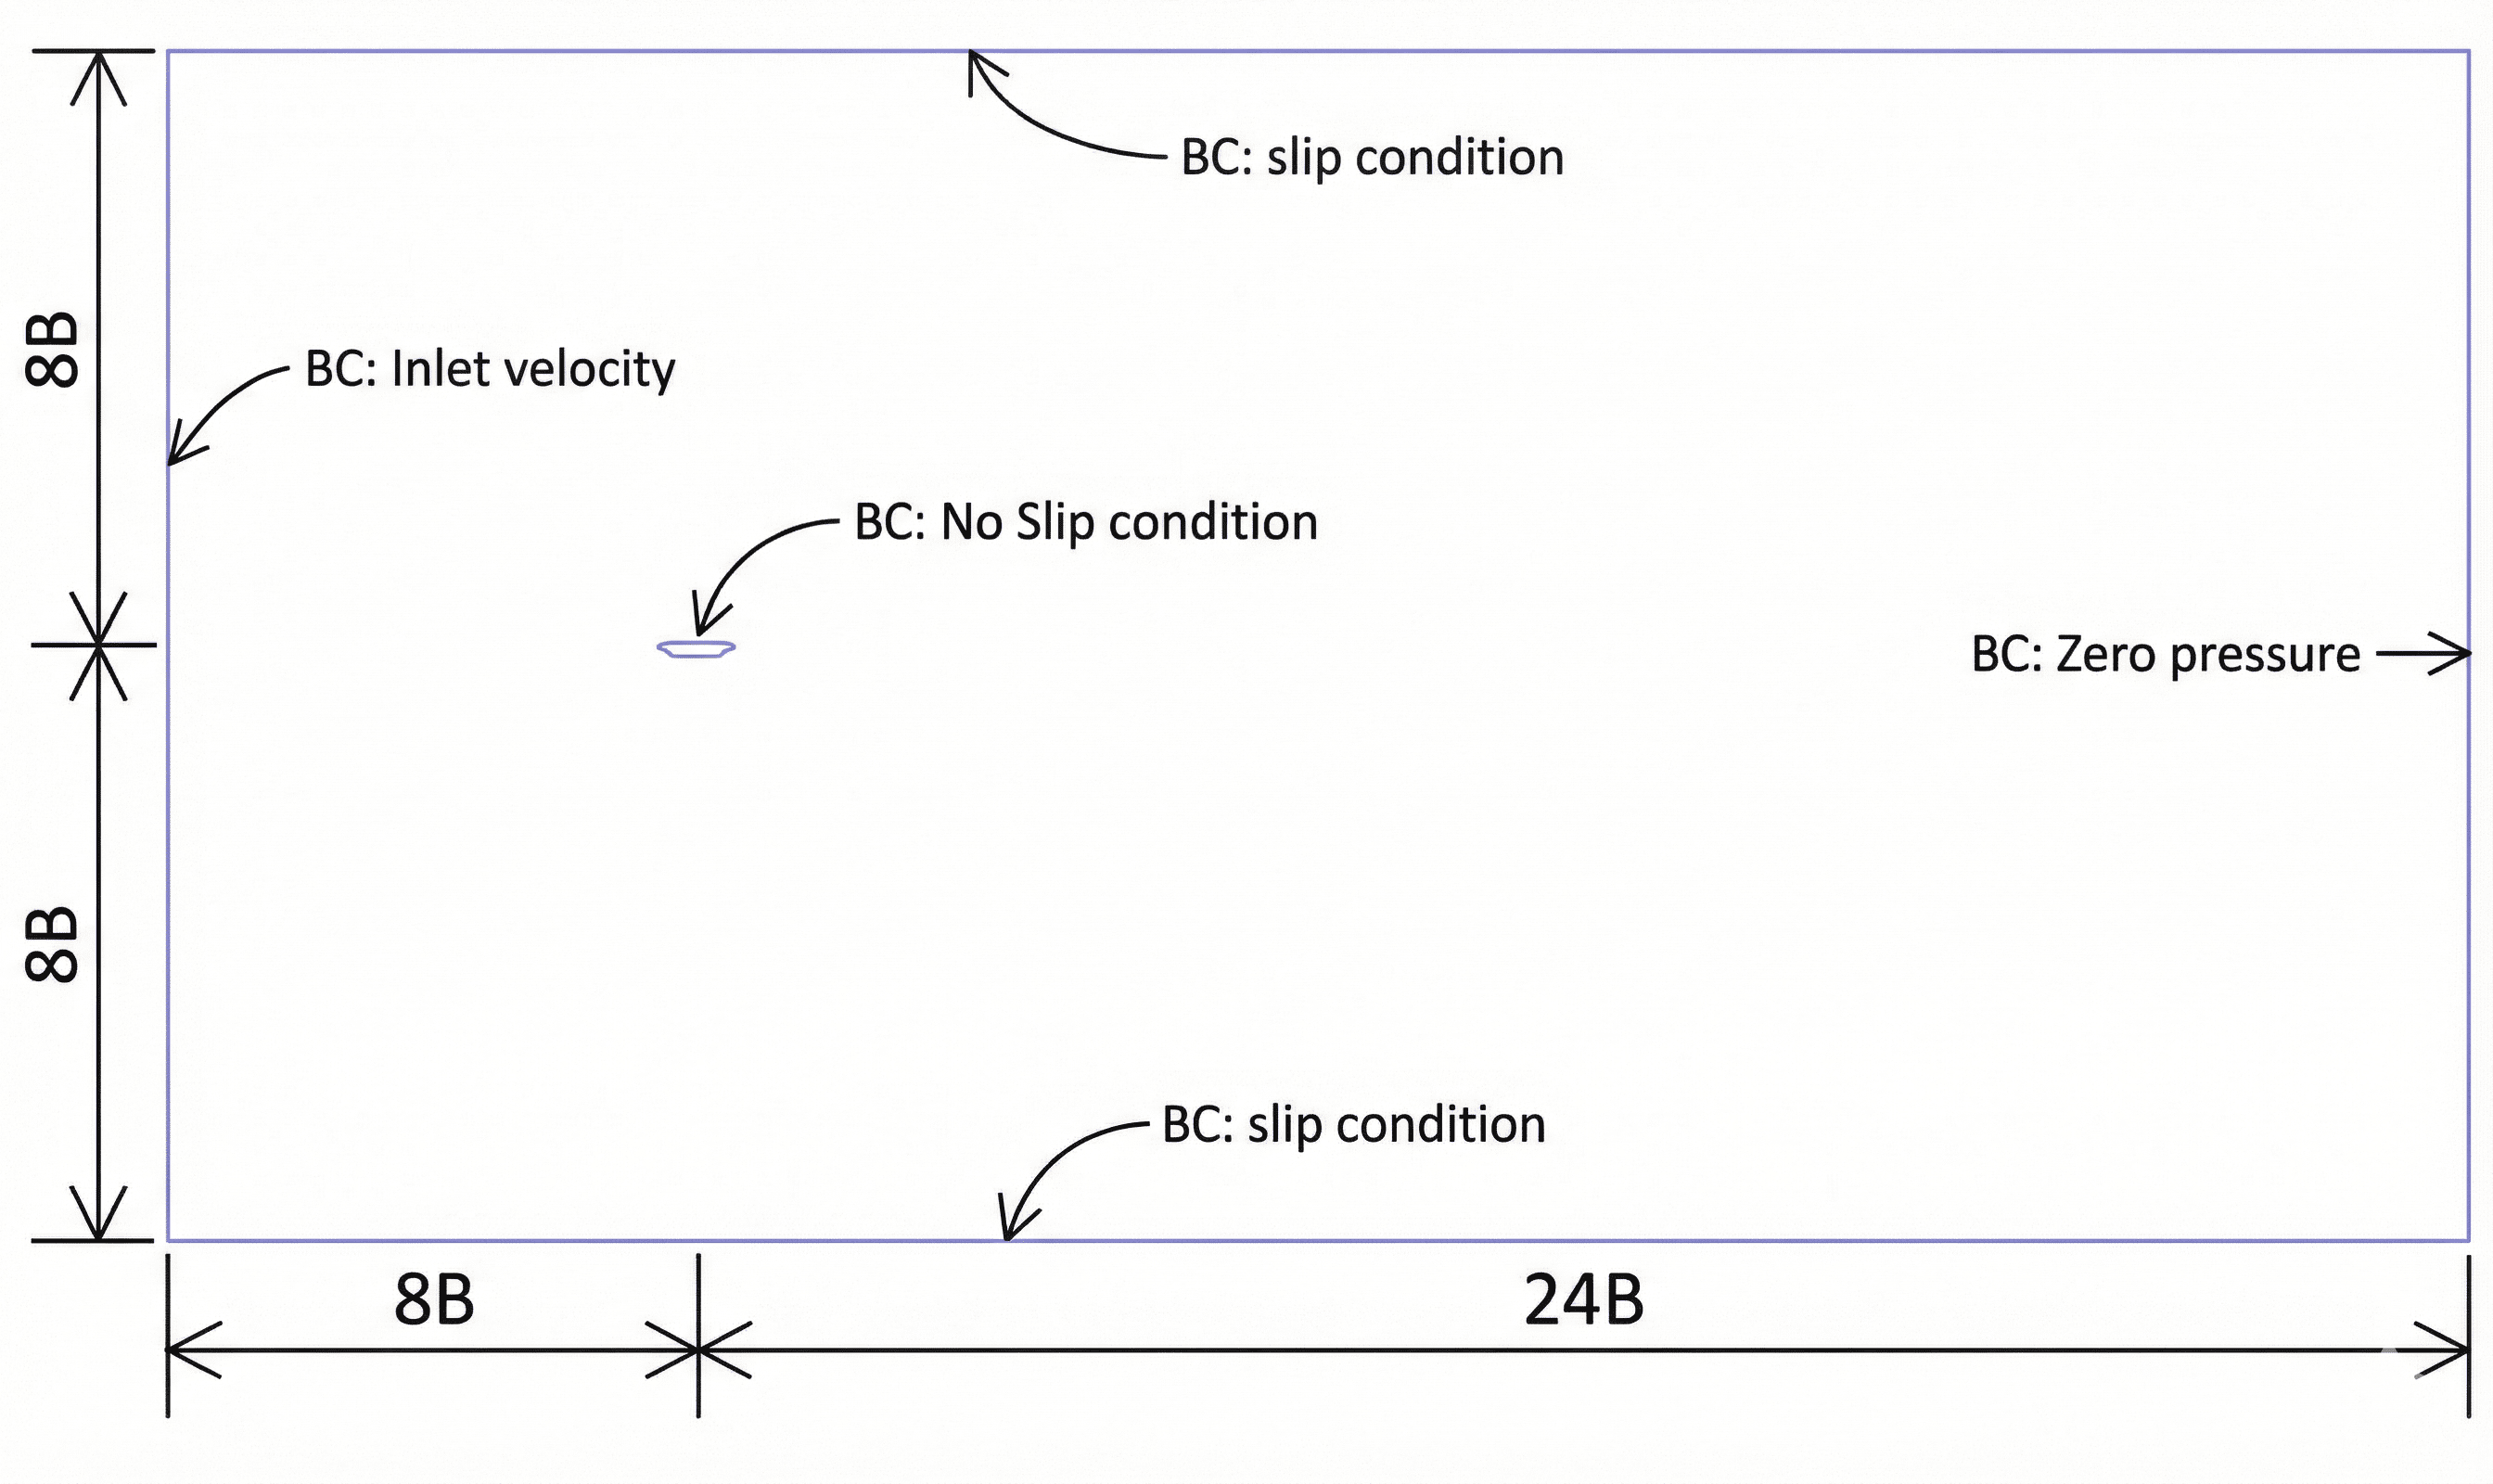
\includegraphics[width=0.65\textwidth]{Figures/Virtual_Wind_Tunnel_Dimensions.png}
    \caption{Virtual Wind Tunnel Dimensions}
    \label{fig:Virtual_Wind_Tunnel_Dimensions}
\end{figure}


\begin{figure}[htbp]  
    \centering
    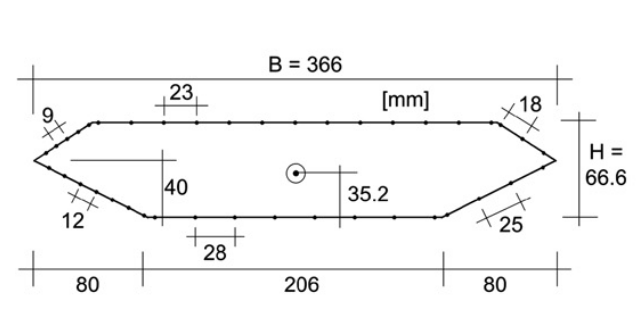
\includegraphics[width=0.5\textwidth]{Figures/Sarkic_Section.png}
    \caption{Sarkic Cross-Section}
    \label{fig:Sarkic_Section}
\end{figure}

\vspace{0.5 cm}

\textbf{Solver Informations:} 

The GiD model is solved with an open source Multiphysics solver - KratosMultiphysics. 
The boundary conditions applied to Fluid domain are shown in Figure~\ref{fig:Virtual_Wind_Tunnel_Dimensions}. 
The turbulence is modeled with URANS and the turbulence intensity is set to 0.1 and the turbulent mixing length is set to 0.0588 m.\\

The velocity is set to 1 m/s and the corresponding Reynolds number for the flow is [insert value]. The time step is 
taken as 0.002 seconds. The total simulation time can be divided into three phases: ramp-up time, stabilization time, and stable 
time period. In Ramp-up phase the flow velocity is steadily increased from 0 to 1 m/s to avoid numerical instabilities. 
In Stabilization phase, the flow is allowed to stabilize. The stable time period is the duration used for analysis. 
Ramp-up time and stabilization time are determined based on the vortex shedding frequency of the section.
From EN 1991, the strouhal number of the section is taken as 0.1. \\ [0.1cm]

Vortex shedding frequency = $ \frac{0.1 * 1}{0.366} $ = 0.273 Hz \\ [0.1cm]
Ramp up time = $ 2 * \frac{1}{0.273} $ = 7.32 seconds \\ [0.1cm]
Stabilization time = $ 2 * \frac{1}{0.273} $ = 7.32 seconds \\ [0.1cm]

The stable time period is for capturing the flow behaviour. Since the interest of this thesis is to capture the flutter response, 
stable time period is time taken for 10 complete forced motion oscillations. But as each reduced velocity 
has a different forced motion frequency, the stable phase of the simulations is different. A higher reduced velocity will 
have a lower oscillating frequency and hence requiring a higher time of simulation and vice versa. Hence its calulcation is 
shown after the information about the applied motion frequency is provided and in the conecutive chapters if anyother 
reduced velocity is taken, the stable time period is mentioned in the respective chapter.

\begin{figure}[htbp]  
    \centering
    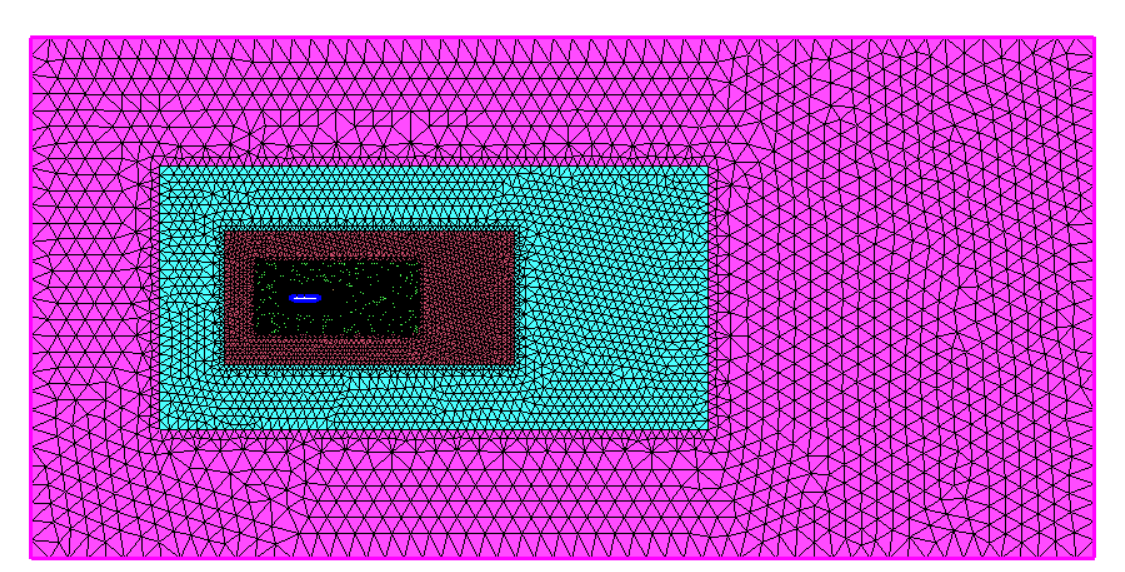
\includegraphics[width=0.65\textwidth]{Figures/GiD_Model_2.png}
    \caption{GiD Model of Virtual Wind Tunnel}
    \label{fig:GiD_Model_2}
\end{figure}

\vspace{0.5 cm}

\textbf{Mesh Convergence Study:} 

A mesh convergence study is conducted to determine the optimal mesh element size. Five models with progressive 
mesh sizes are created and converegence of 8 derivatives are analysed. The Table~\ref{tab:mesh_convergence} shows the models
and corresponding mesh sizes at each zone. The study is performed for a single point on the flutter derivative curve
at a reduced velocity of 10.93. From the literature, reivew, it is identified 5$\%$ of width of bridge deck as the heave amplitude 
and 5 degree as pitch amplitude are the appropiate forced motion amplitude such that aerodynamic forces show linear behaviour.  \\ [0.1cm]

Heave amplitude = $ \frac{5 * 0.366}{100} $ = 0.0183 m\\ [0.1cm]
Pitch amplitude = 0.087 radians\\ [0.1cm]
Motion Frequency = 0.25 Hz\\ [0.1cm] 
Stable time period = $ 10 * \frac{1}{0.25} $ = 40 seconds\\ [0.1cm]
Total simulation time = Ramp-up time + Stabilization time + Stable time period = 7.32 + 7.32 + 40 = 54.64 seconds\\ [0.1cm]


\begin{table}[htbp]  
    \centering
    \caption{Mesh Convergence Study Results}
    \label{tab:mesh_convergence}
    \begin{tabular}{|l|c|c|c|c|c|}
        \hline
        \textbf{} & \textbf{Model 1} & \textbf{Model 2} & \textbf{Model 3} & \textbf{Model 4} & \textbf{Model 5} \\ \hline
        Zone A (m) & 0.25 & 0.25 & 0.2304 & 0.2112 & 0.192 \\ \hline
        Zone B (m) & 0.1 & 0.12 & 0.1152 & 0.1056 & 0.096 \\ \hline
        Zone C (m) & 0.054 & 0.08 & 0.0576 & 0.0528 & 0.048 \\ \hline
        Zone D (m) & 0.018 & 0.025 & 0.0288 & 0.0264 & 0.024 \\ \hline
        Zone E (m) & - & - & 0.0096 & 0.0088 & 0.008 \\ \hline
        Zone F (m) & 0.009 & 0.008 & 0.0048 & 0.0044 & 0.004 \\ \hline
        Deck Surface (m) & 0.0045 & 0.003 & 0.0024 & 0.0022 & 0.002 \\ \hline
        Width/ min mesh size & 81.333 & 122 & 152.5 & 166.36 & 183 \\ \hline
        Total Elements & 7368 & 15704 & 20854 & 24374 & 29408 \\ \hline
        Minimum Mesh Size GID & 0.00358 & 0.00245 & 0.00196 & 0.00179 & 0.00159 \\ \hline
        Velocity (m/s) & 1 & 1 & 1 & 1 & 1 \\ \hline
        Time step & 0.004 & 0.002 & 0.002 & 0.002 & 0.002 \\ \hline
        CFL & 1.11 & 0.81 & 1.02 & 1.11 & 1.26 \\ \hline
    \end{tabular}
\end{table}

With this simulation setup, the CFD simulations are conducted for all five models figure~\ref{fig:CFD_Result}. 
This maginitude of heave and pitch amplitudes are applied and corrresponding aerodynamic lift and moment
forces are indentified. The aerodynamic forces are then used to calculate the flutter derivatives. The convergence of flutter derivatives is then analysed. 
Figure~\ref{fig:Model_3_CFD_Output} shows the aerodynamic lift and moment forces obtained for Model 3. 


\begin{figure}[htbp]  
    \centering
    
\includegraphics[width=1\textwidth]{Figures/CFD_Result.png}
    \caption{CFD Results for Model 3}
    \label{fig:CFD_Result}
\end{figure}

\vspace{0.5 cm}

\begin{figure}[htbp]
    \centering
    \begin{subfigure}{\textwidth}
        \centering
        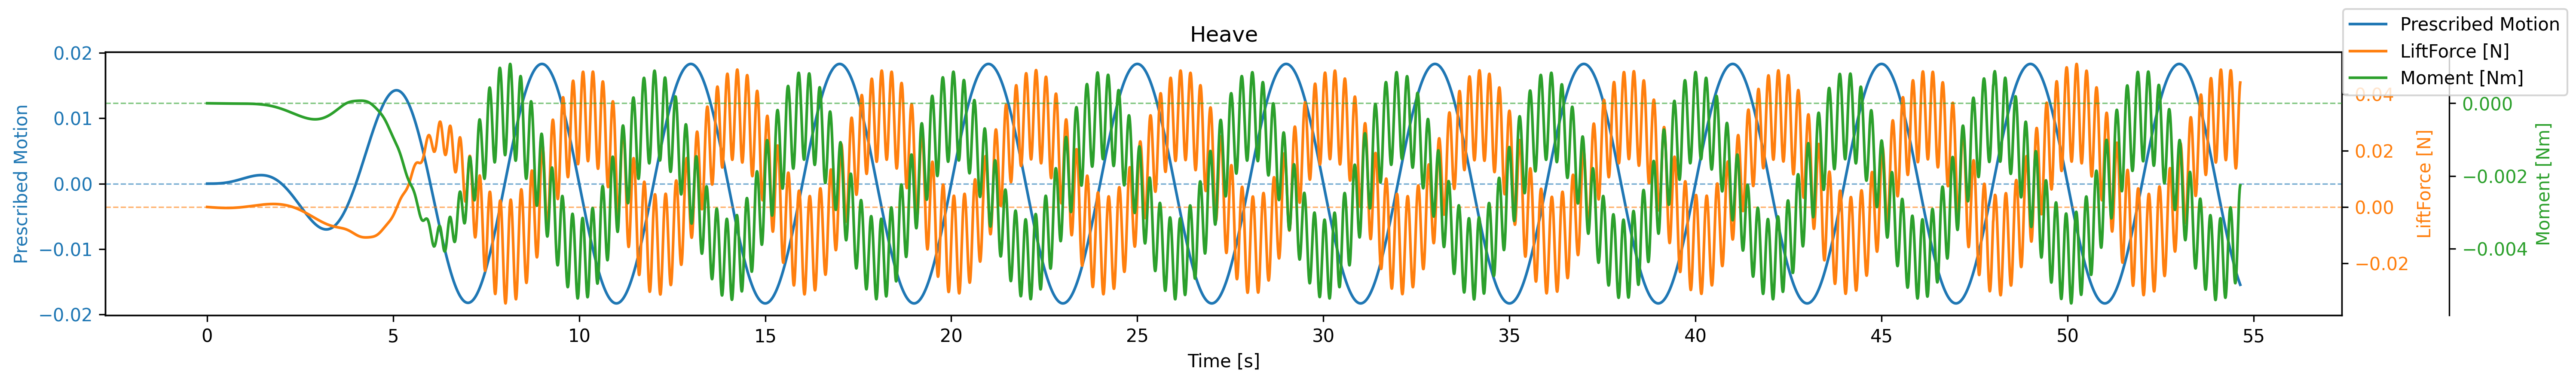
\includegraphics[width=1\textwidth]{Figures/Model_3_Heave.png}
        \caption{Heave}
        \label{fig:Heave}
    \end{subfigure}
    \vspace{0.5cm}
    \begin{subfigure}{\textwidth}
        \centering
        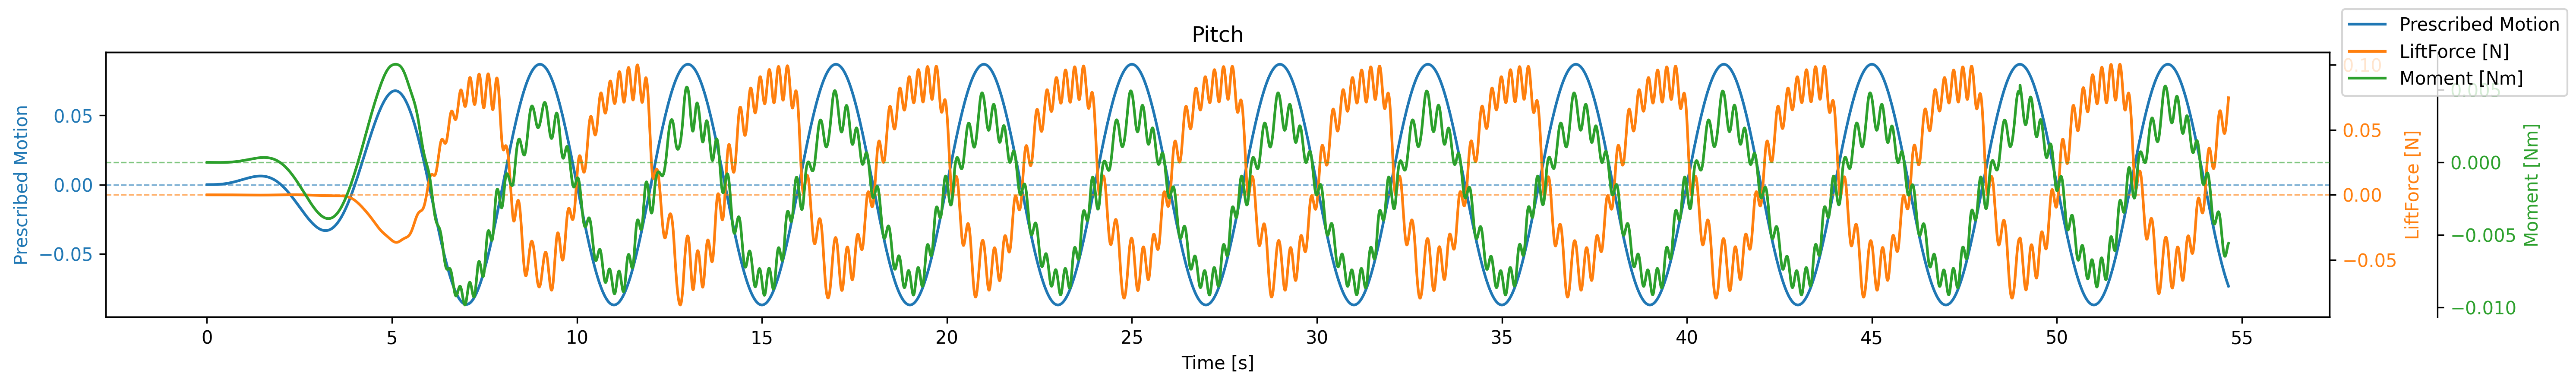
\includegraphics[width=1\textwidth]{Figures/Model_3_Pitch.png}
        \caption{}Pitch
        \label{fig:Pitch}
    \end{subfigure}
    \caption{Heave Motion}
    \label{fig:Model_3_CFD_Output}
\end{figure}

The results of the mesh convergence study are shown in Figure~\ref{fig:convergence}. It is observed that the 
derivatives $H_1,H_3,A_1,A_2,$ and $A_3$ exhibited good convergence, while derivatives  $H_2,H_4,$ and $A_4$ displayed 
oscillatory convergence behavior. This behavior is consistent with findings in the literature, as these 
particular derivatives are known to be more difficult to capture accurately. From the study it is concluded, 
Model 3 is optimal and this mesh size is used for all subsequent simulations.

%% Figures for Mesh Convergence Study
\begin{figure}[htbp]  
    \centering
    \begin{subfigure}[b]{0.45\textwidth}
        \centering
        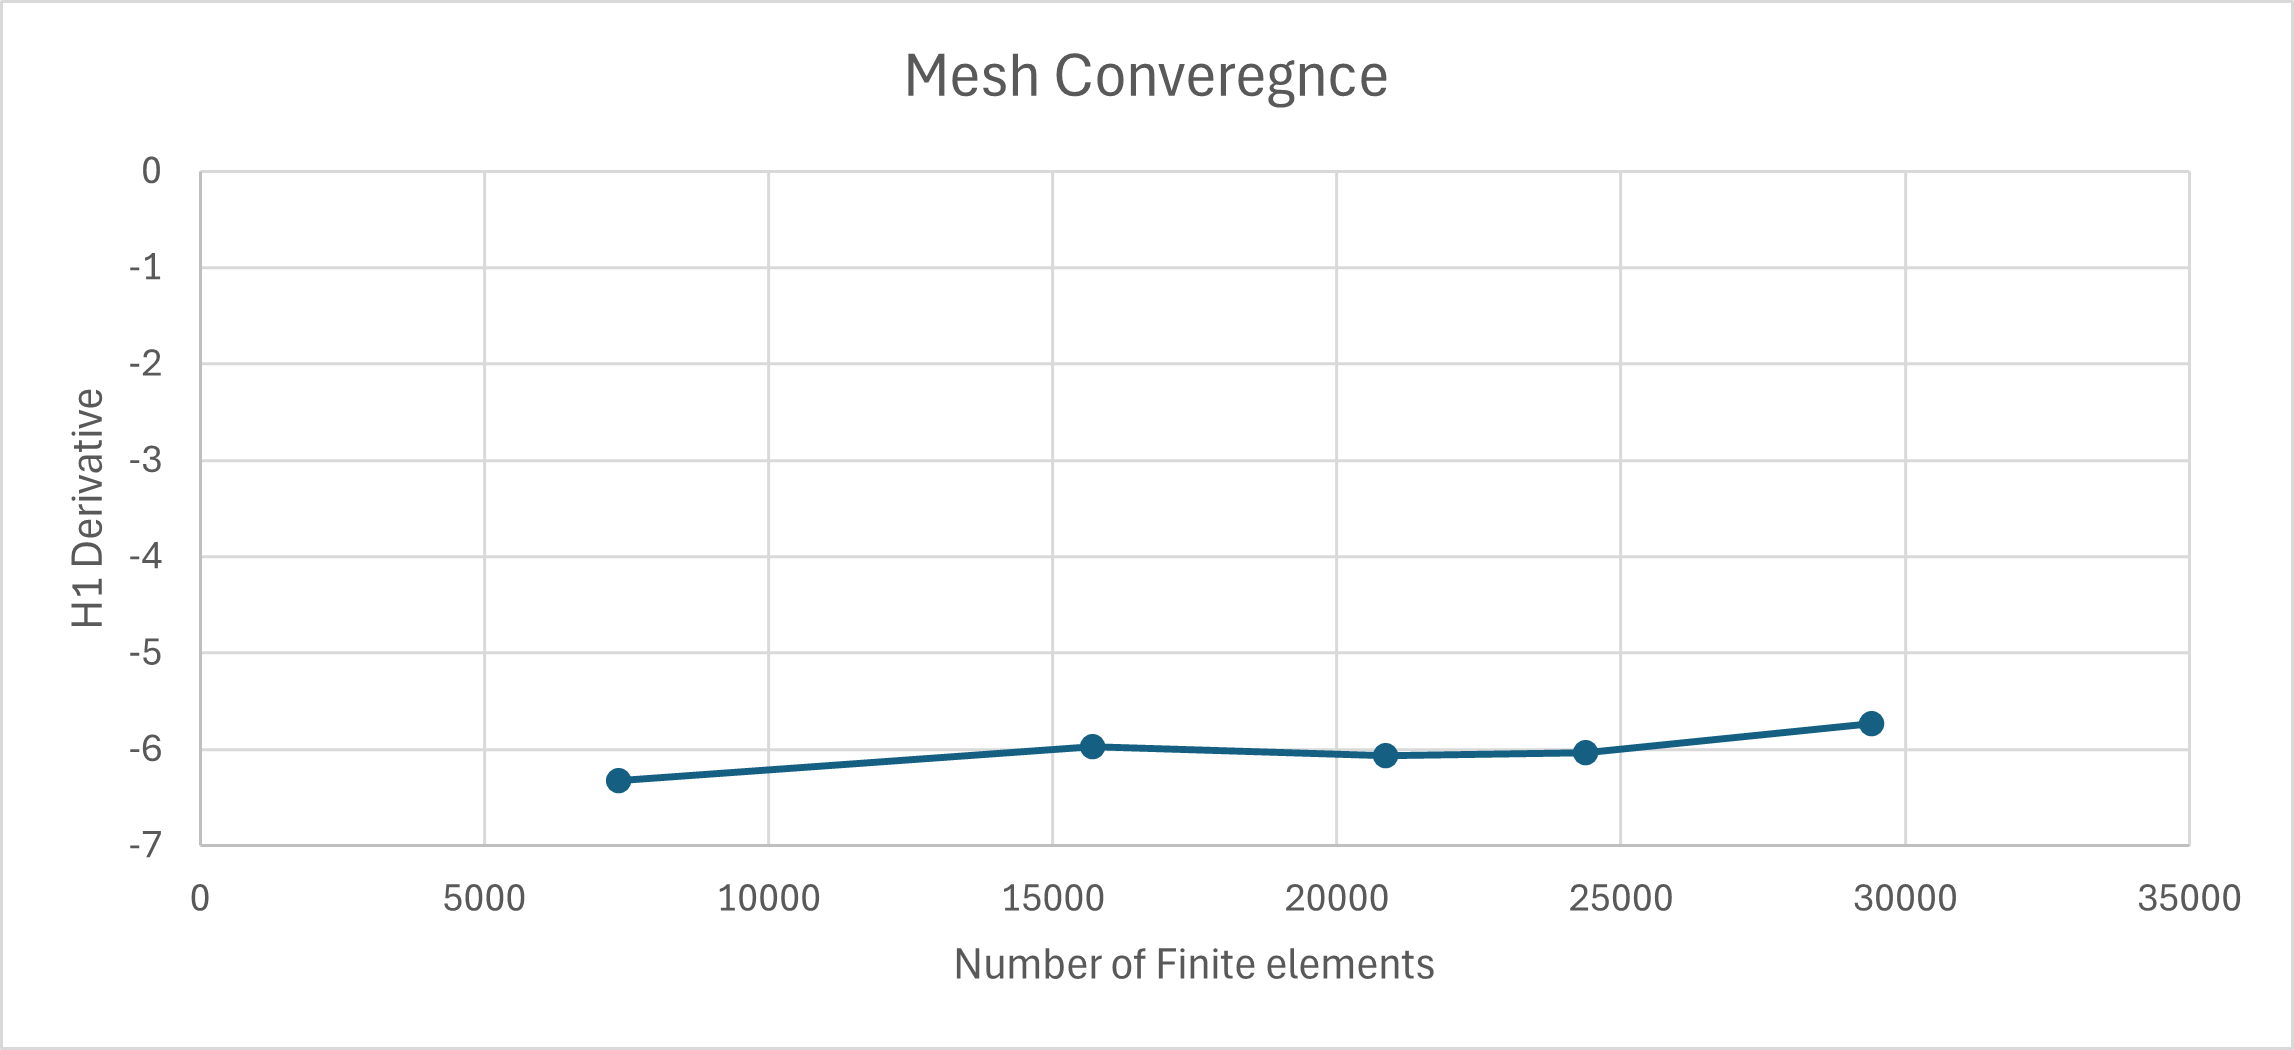
\includegraphics[width=\textwidth]{Figures/Convergence_Study_H1}
        \caption{H1}
        \label{fig:h1}
    \end{subfigure}
    \hfill
    \begin{subfigure}[b]{0.45\textwidth}
        \centering
        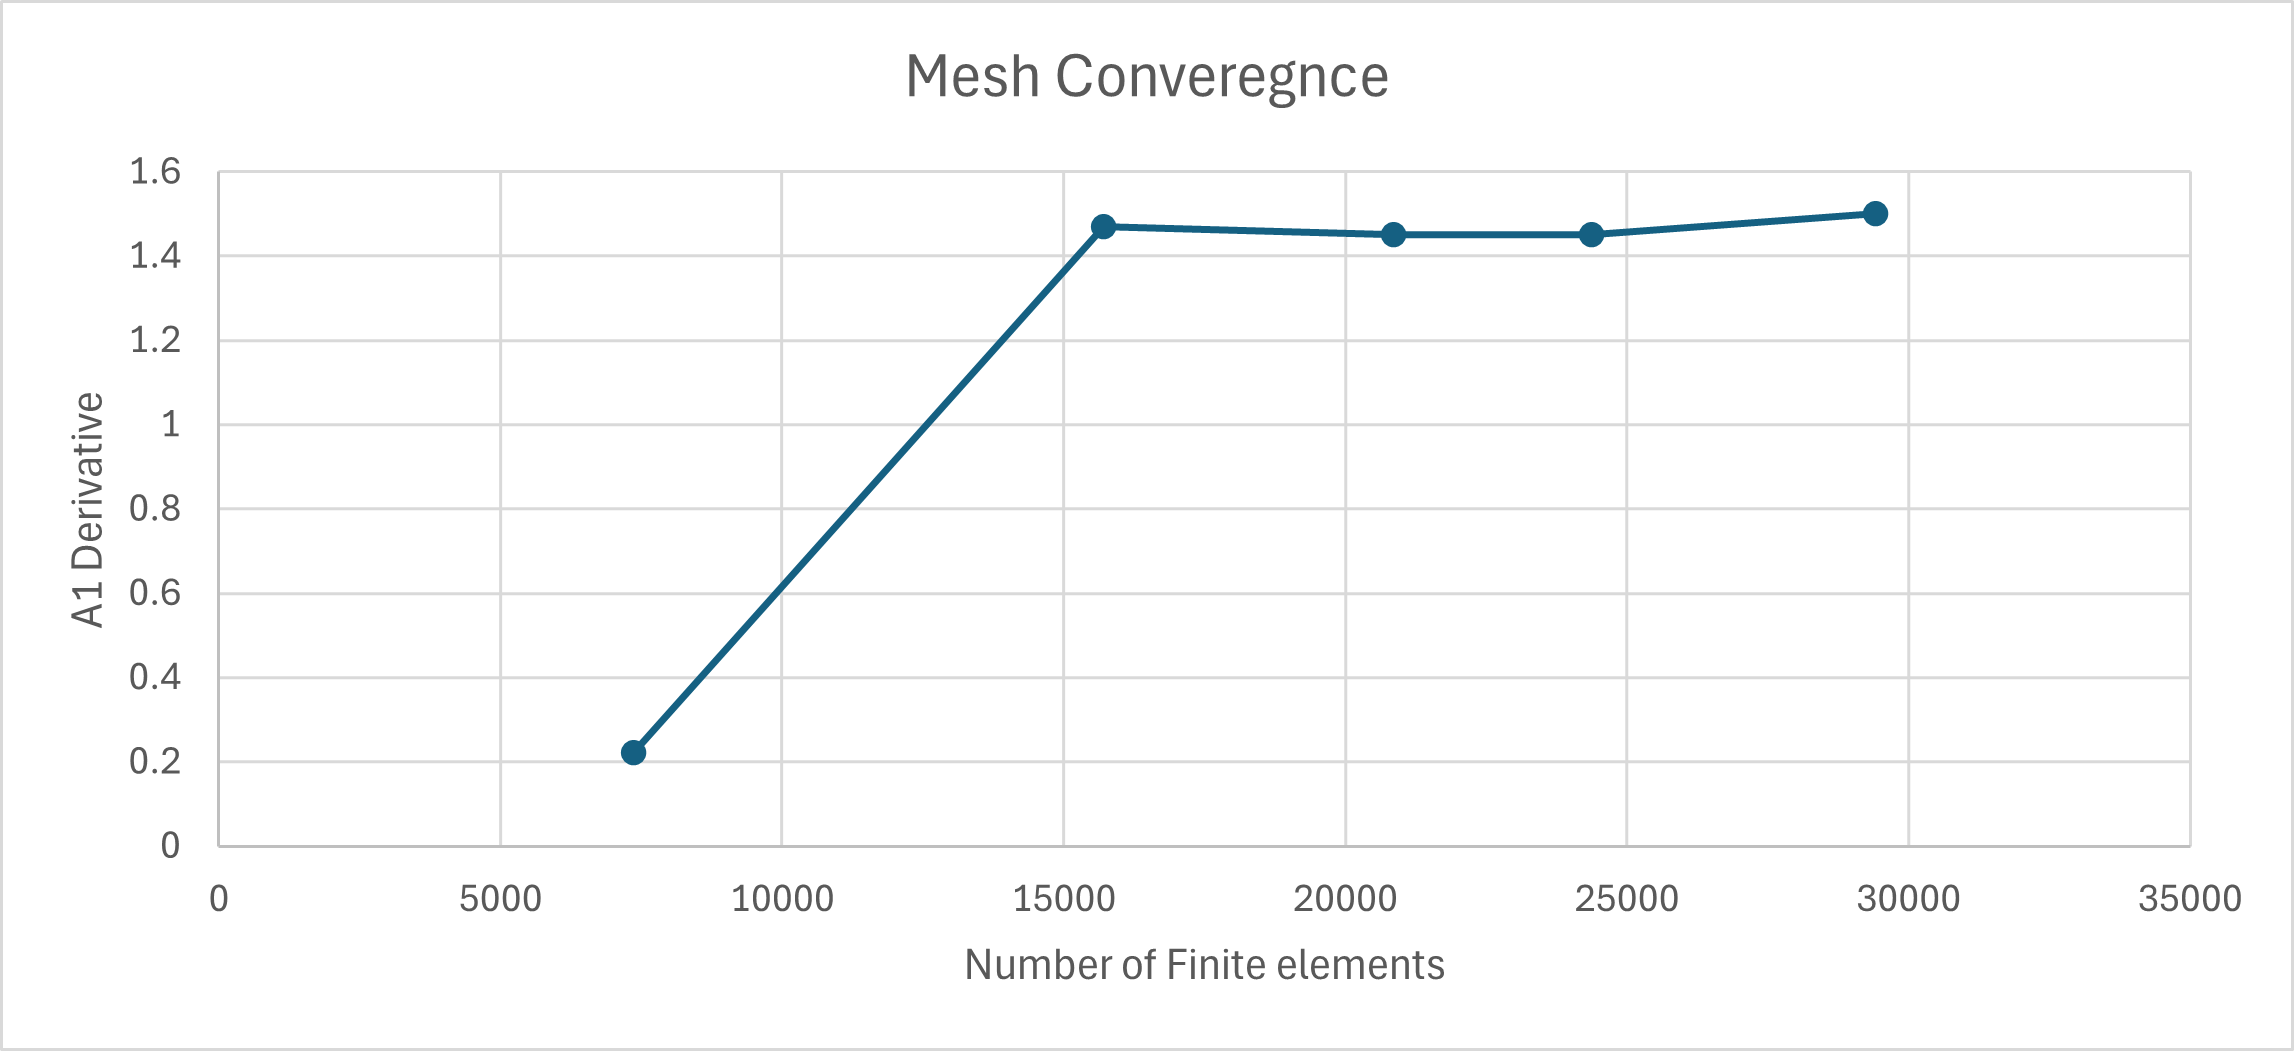
\includegraphics[width=\textwidth]{Figures/Convergence_Study_A1}
        \caption{A1}
        \label{fig:a1}
    \end{subfigure}
    
    \begin{subfigure}[b]{0.45\textwidth}
        \centering
        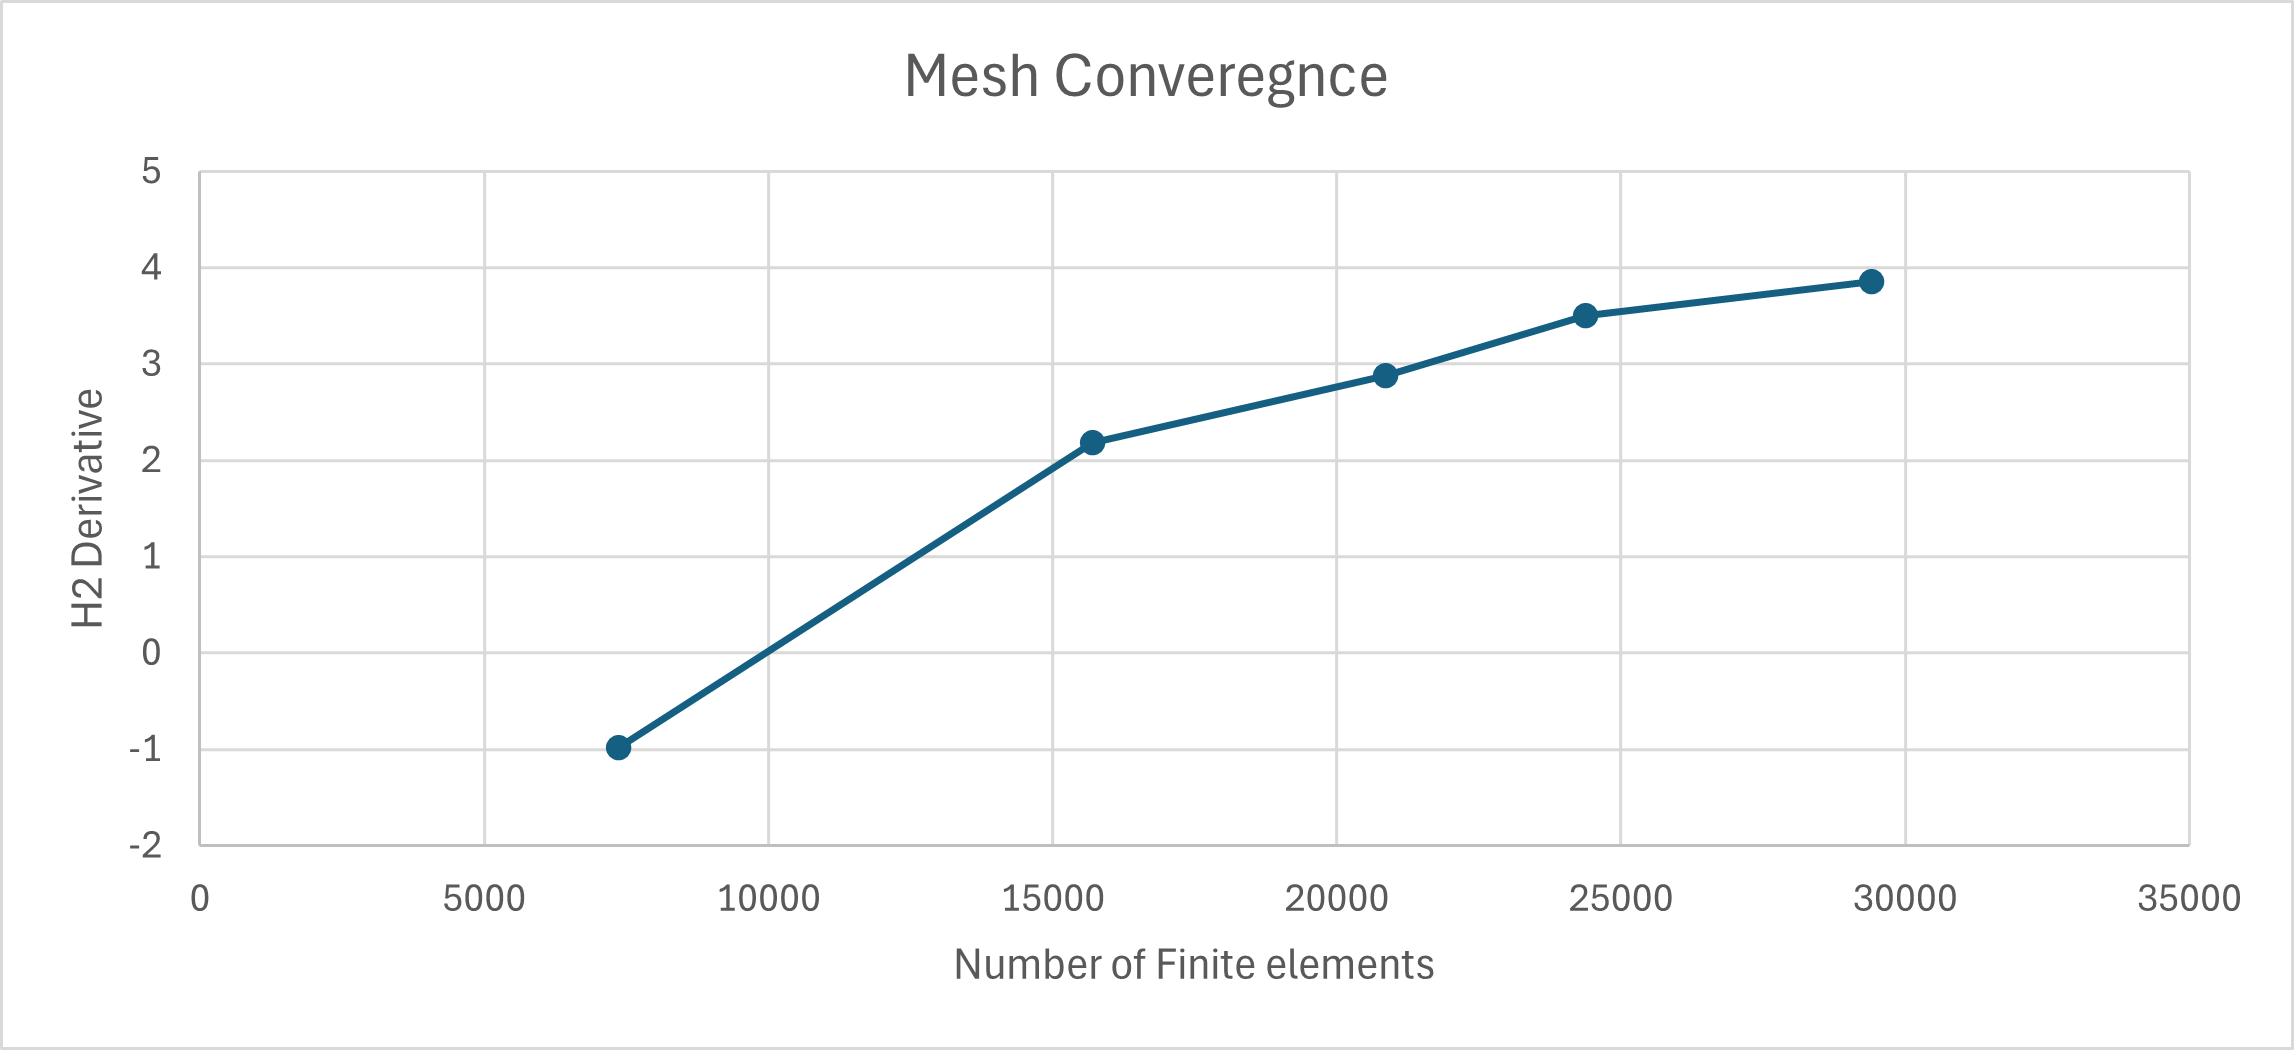
\includegraphics[width=\textwidth]{Figures/Convergence_Study_H2}
        \caption{H2}
        \label{fig:h2}
    \end{subfigure}
    \hfill
    \begin{subfigure}[b]{0.45\textwidth}
        \centering
        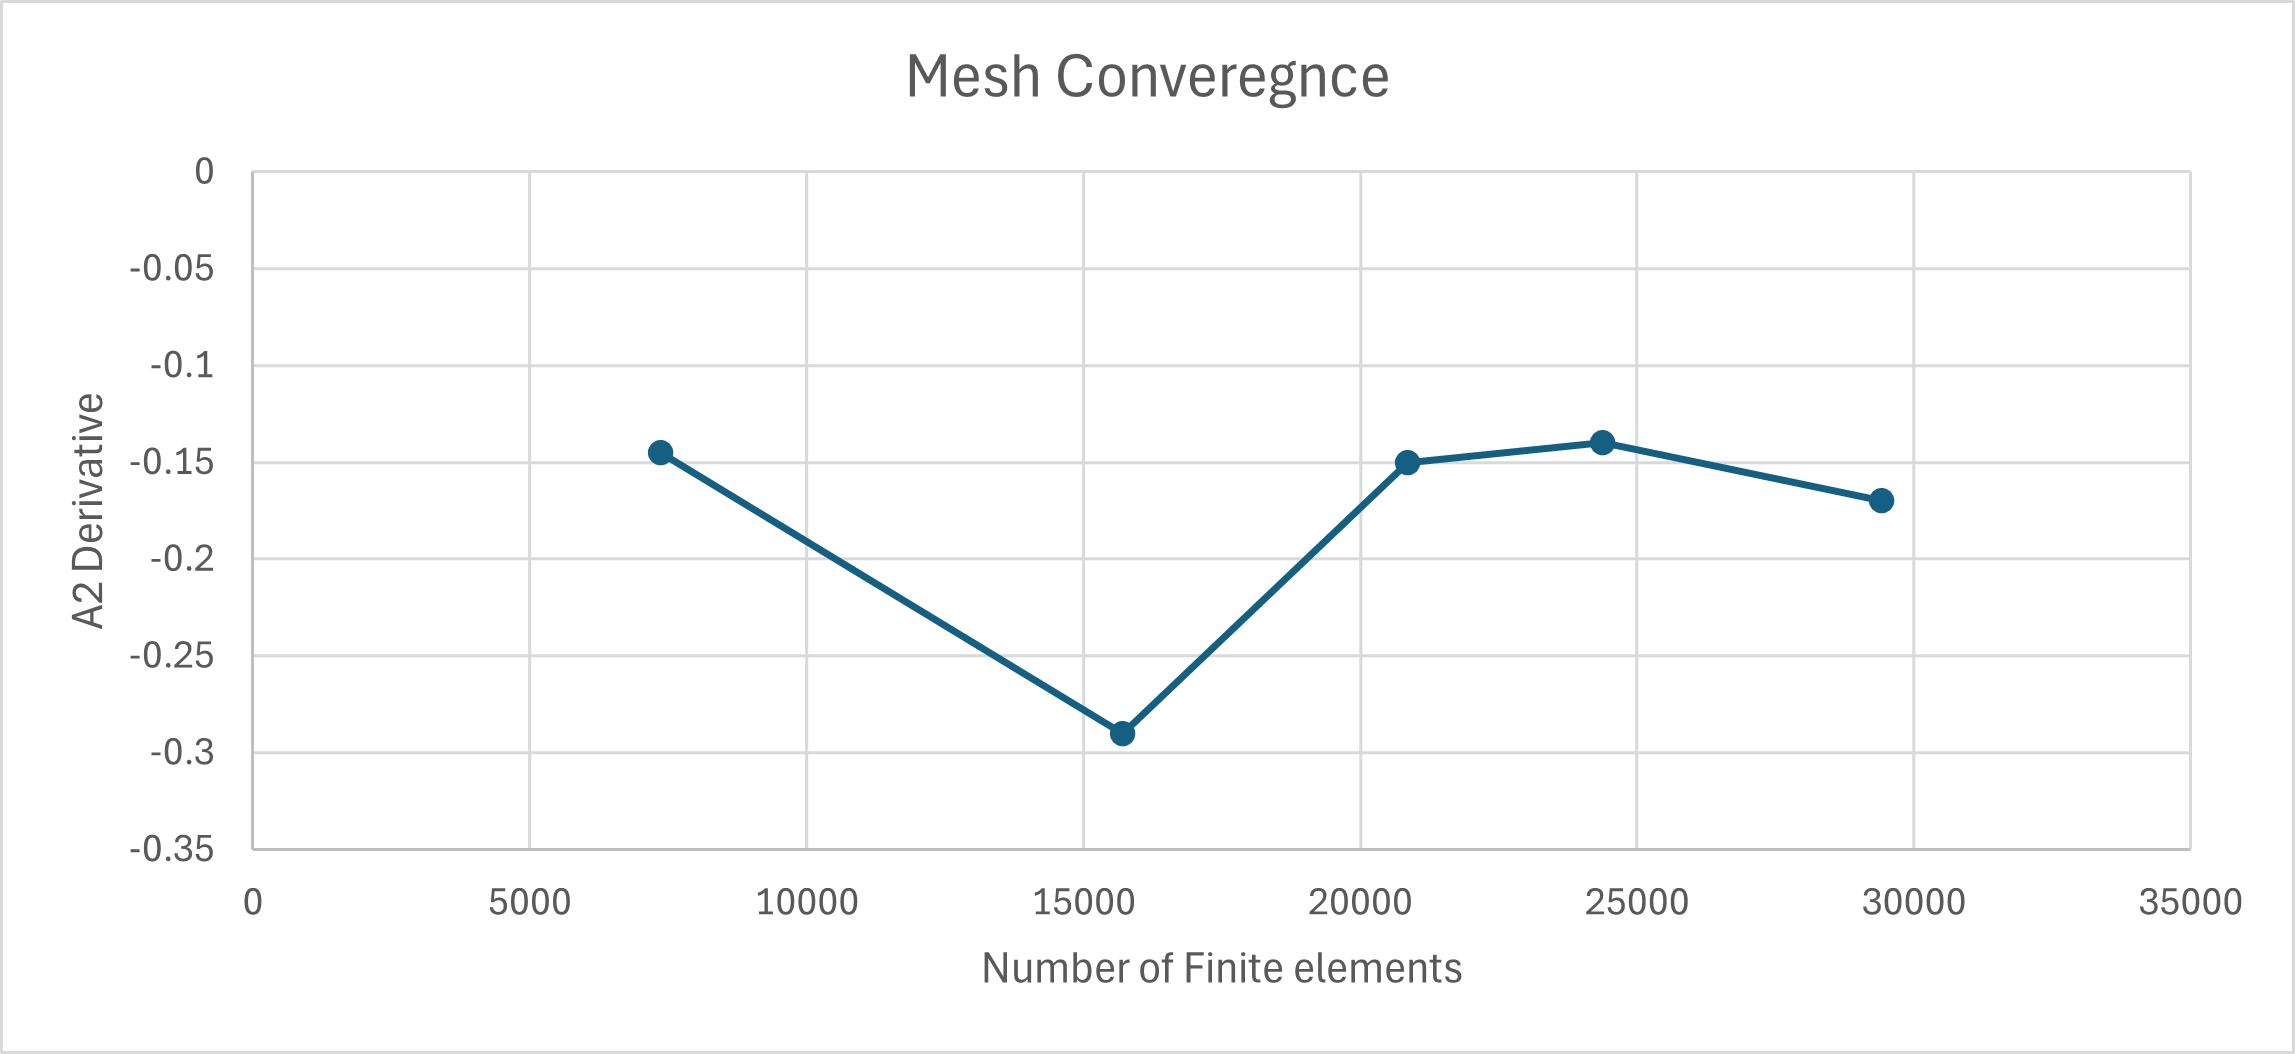
\includegraphics[width=\textwidth]{Figures/Convergence_Study_A2}
        \caption{A2}
        \label{fig:a2}
    \end{subfigure}
    
    \begin{subfigure}[b]{0.45\textwidth}
        \centering
        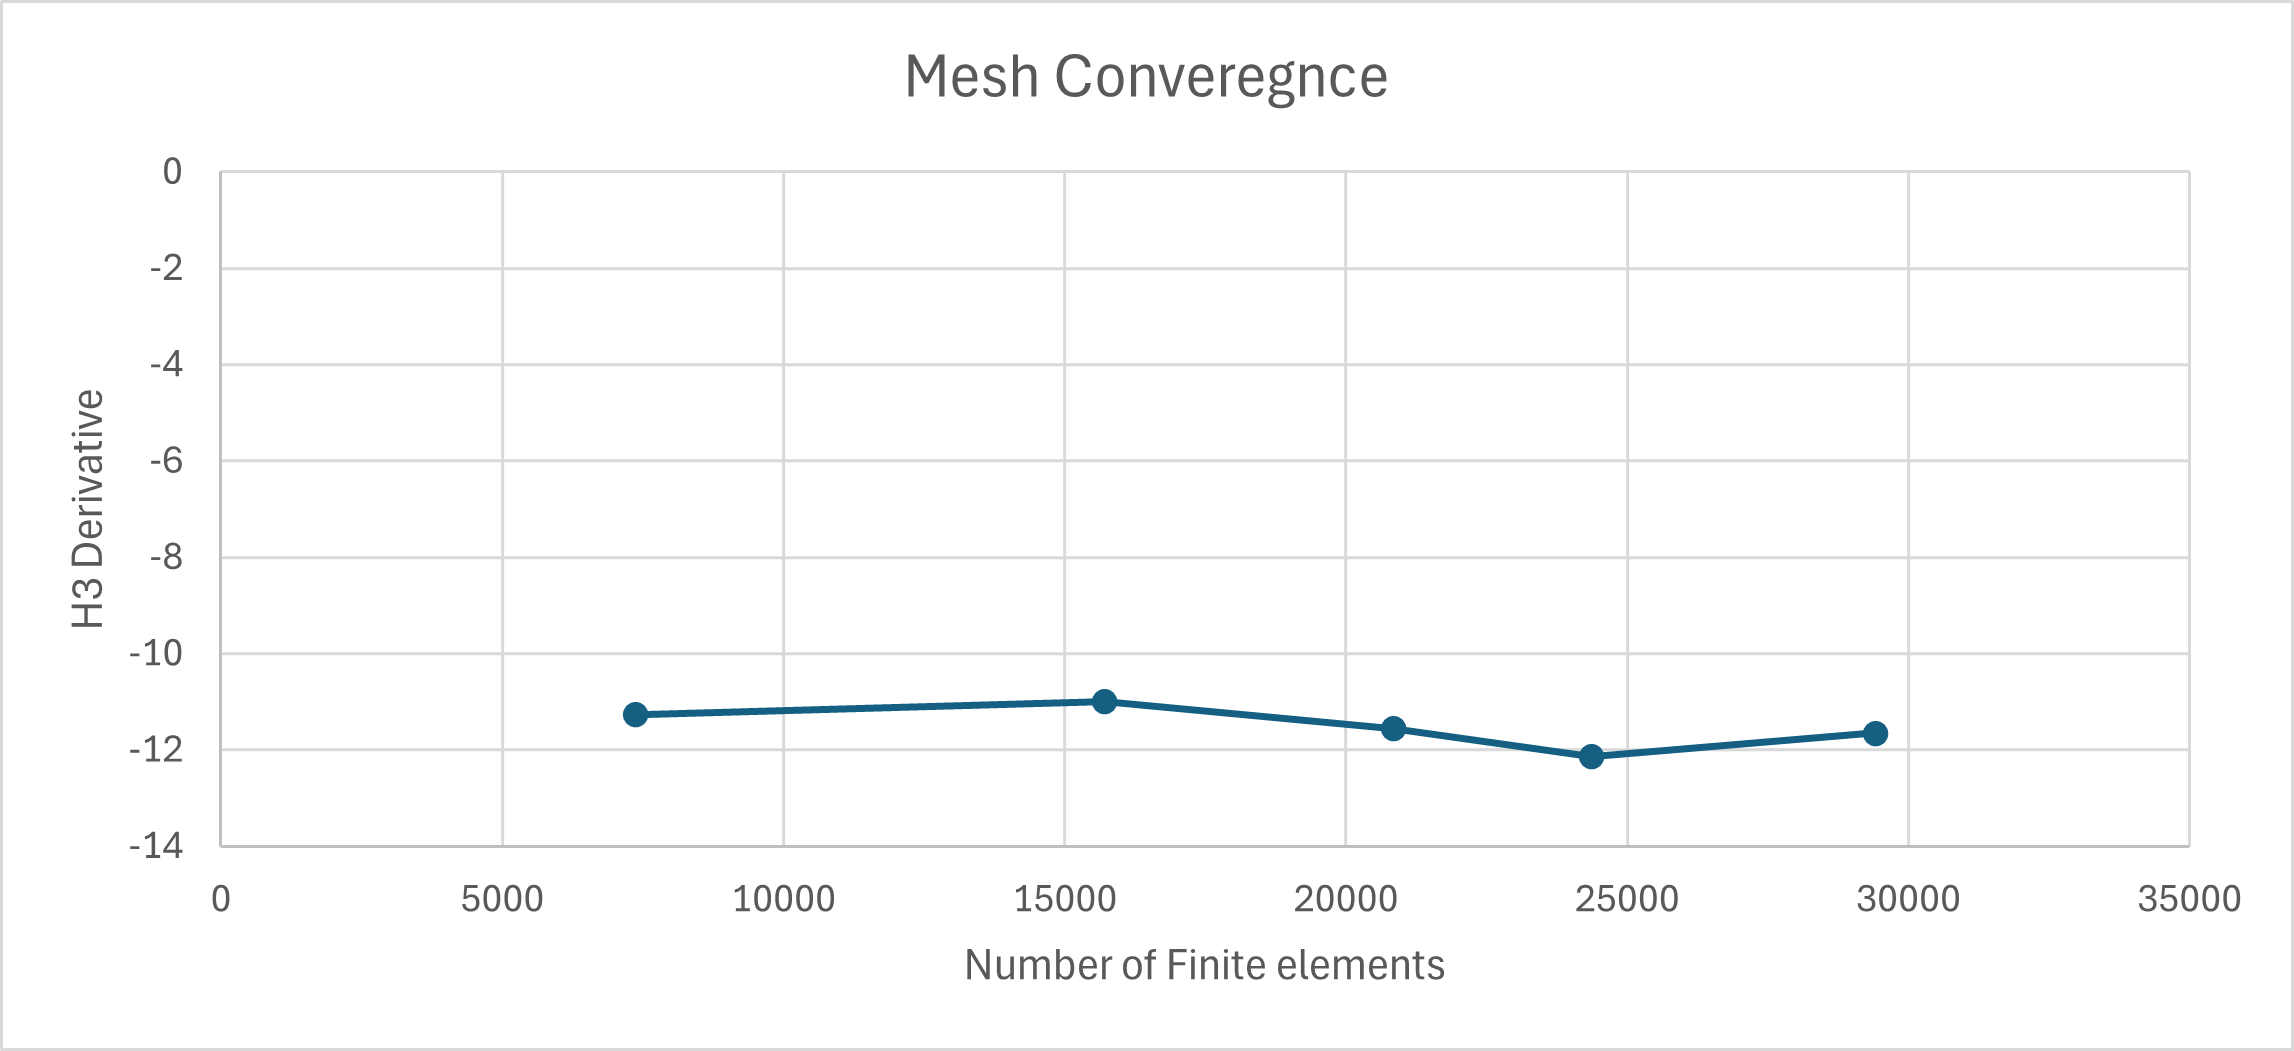
\includegraphics[width=\textwidth]{Figures/Convergence_Study_H3}
        \caption{H3}
        \label{fig:h3}
    \end{subfigure}
    \hfill
    \begin{subfigure}[b]{0.45\textwidth}
        \centering
        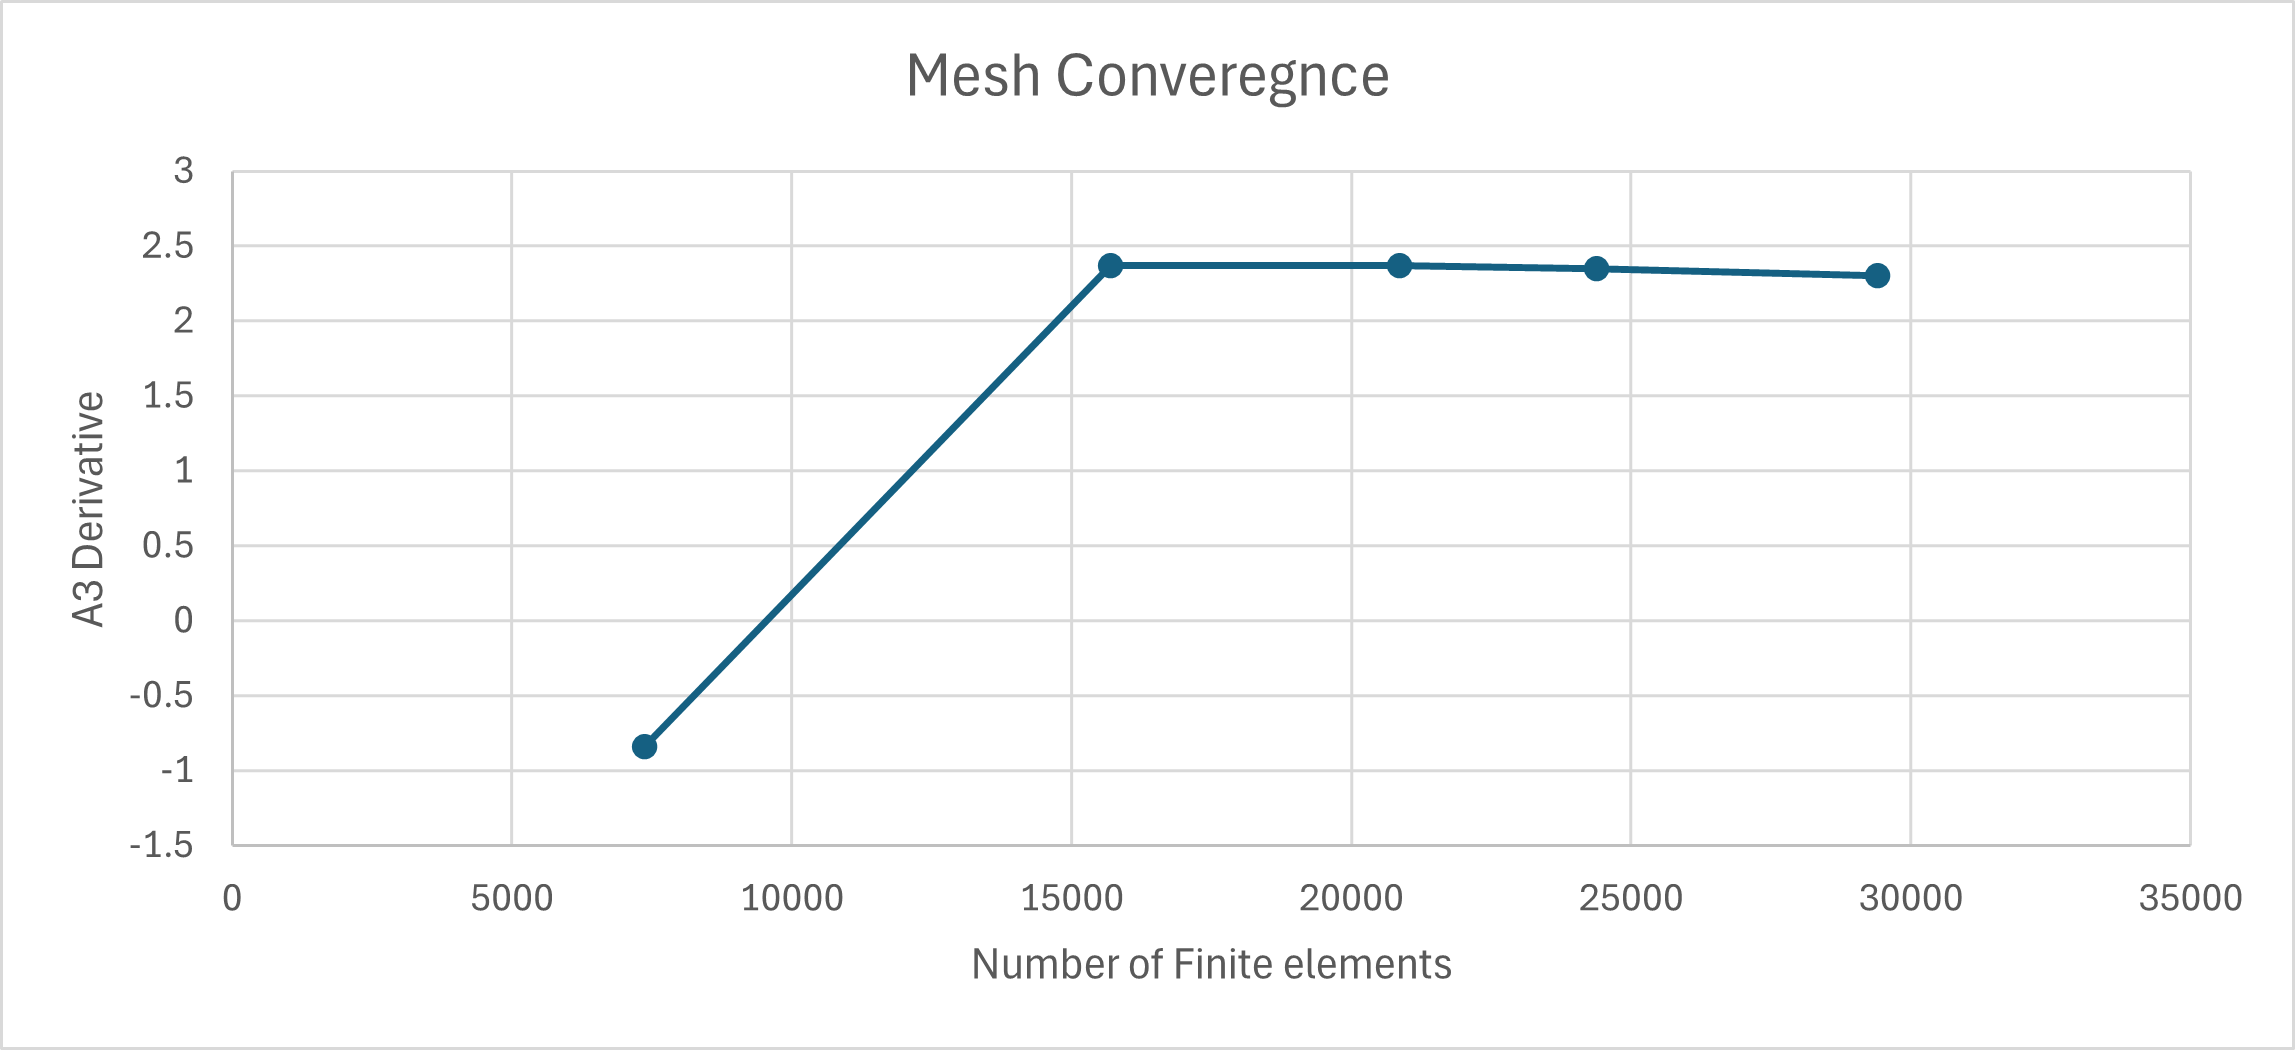
\includegraphics[width=\textwidth]{Figures/Convergence_Study_A3}
        \caption{A3}
        \label{fig:a3}
    \end{subfigure}
    
    \begin{subfigure}[b]{0.45\textwidth}
        \centering
        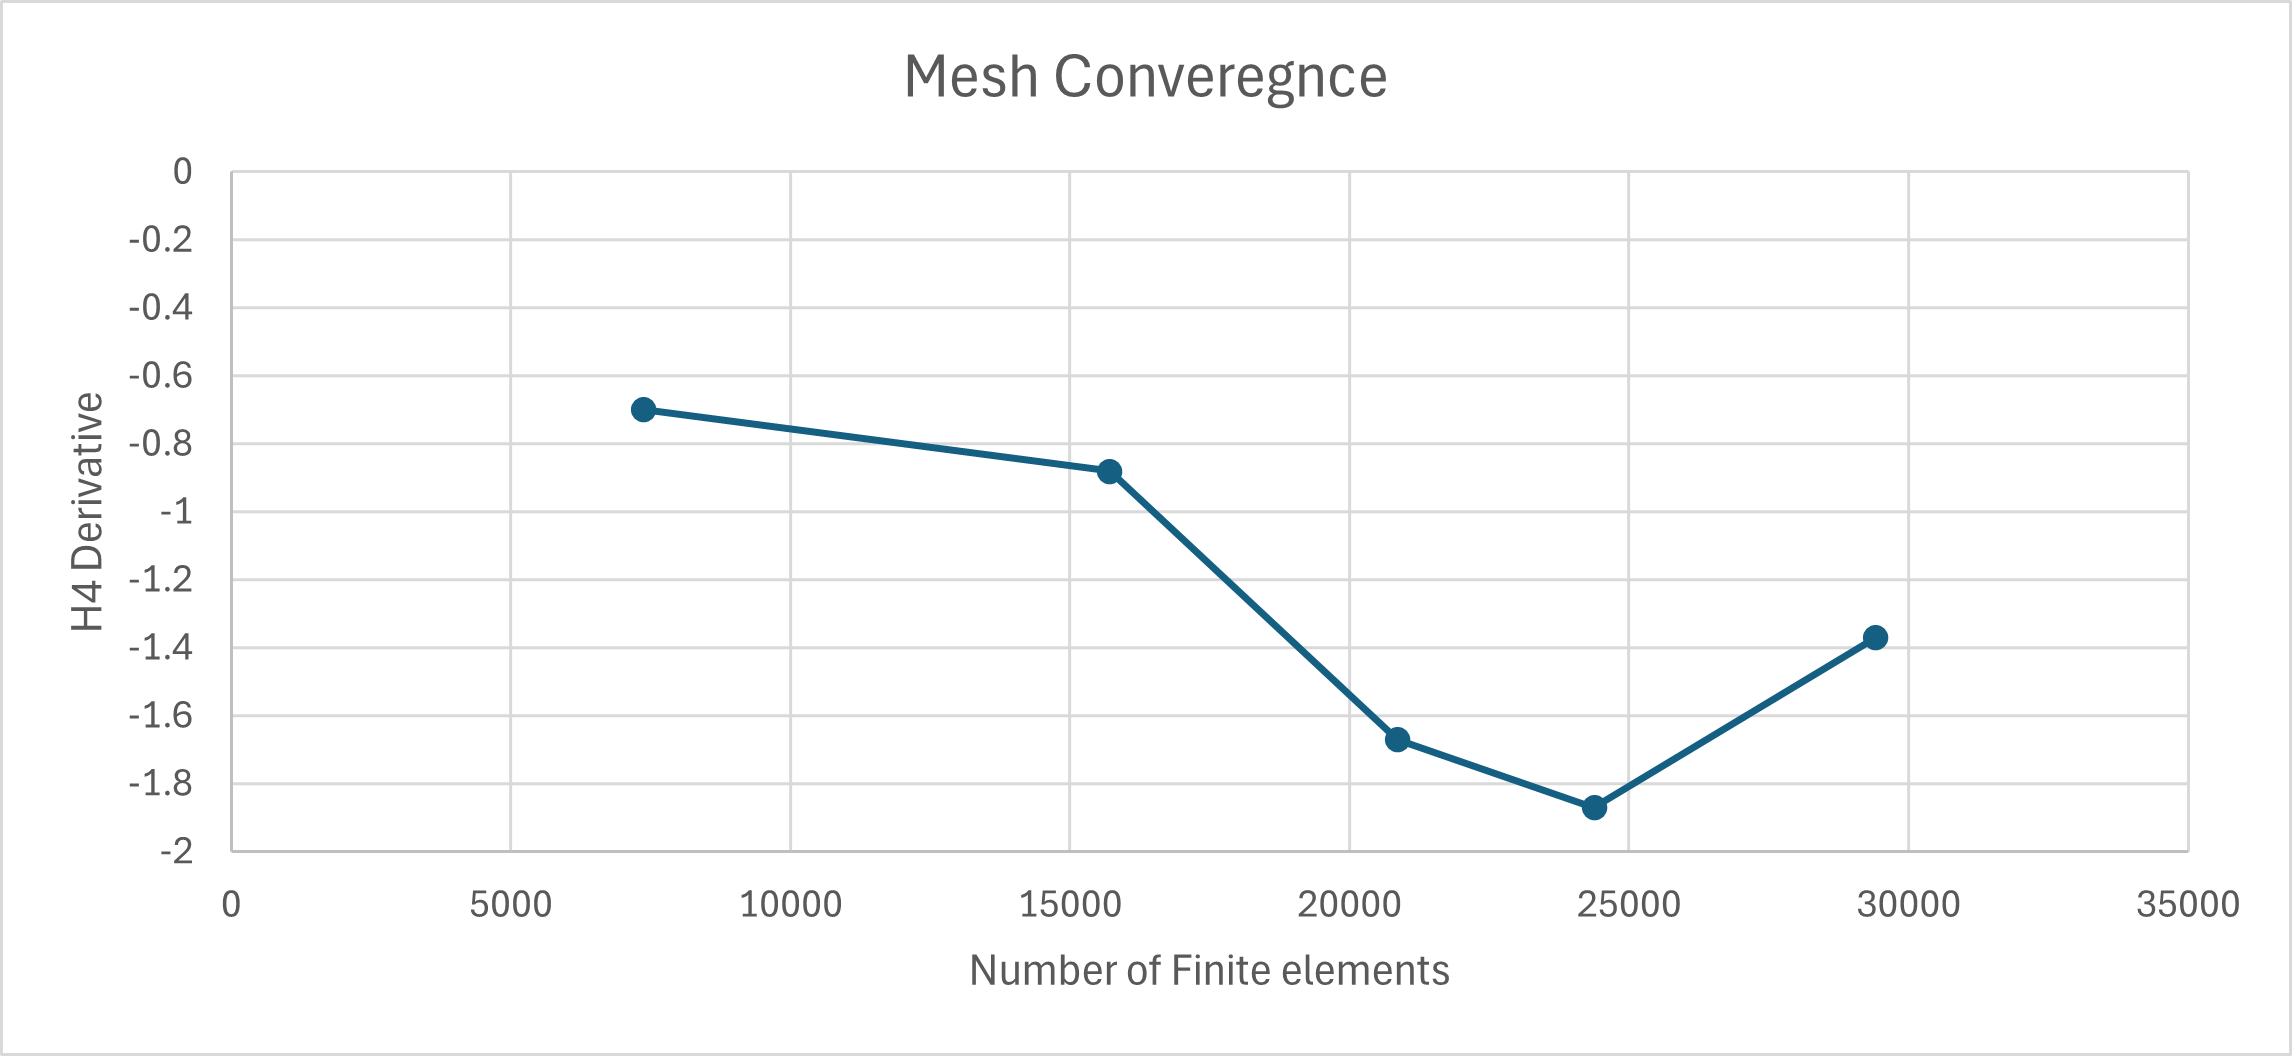
\includegraphics[width=\textwidth]{Figures/Convergence_Study_H4}
        \caption{H4}
        \label{fig:h4}
    \end{subfigure}
    \hfill
    \begin{subfigure}[b]{0.45\textwidth}
        \centering
        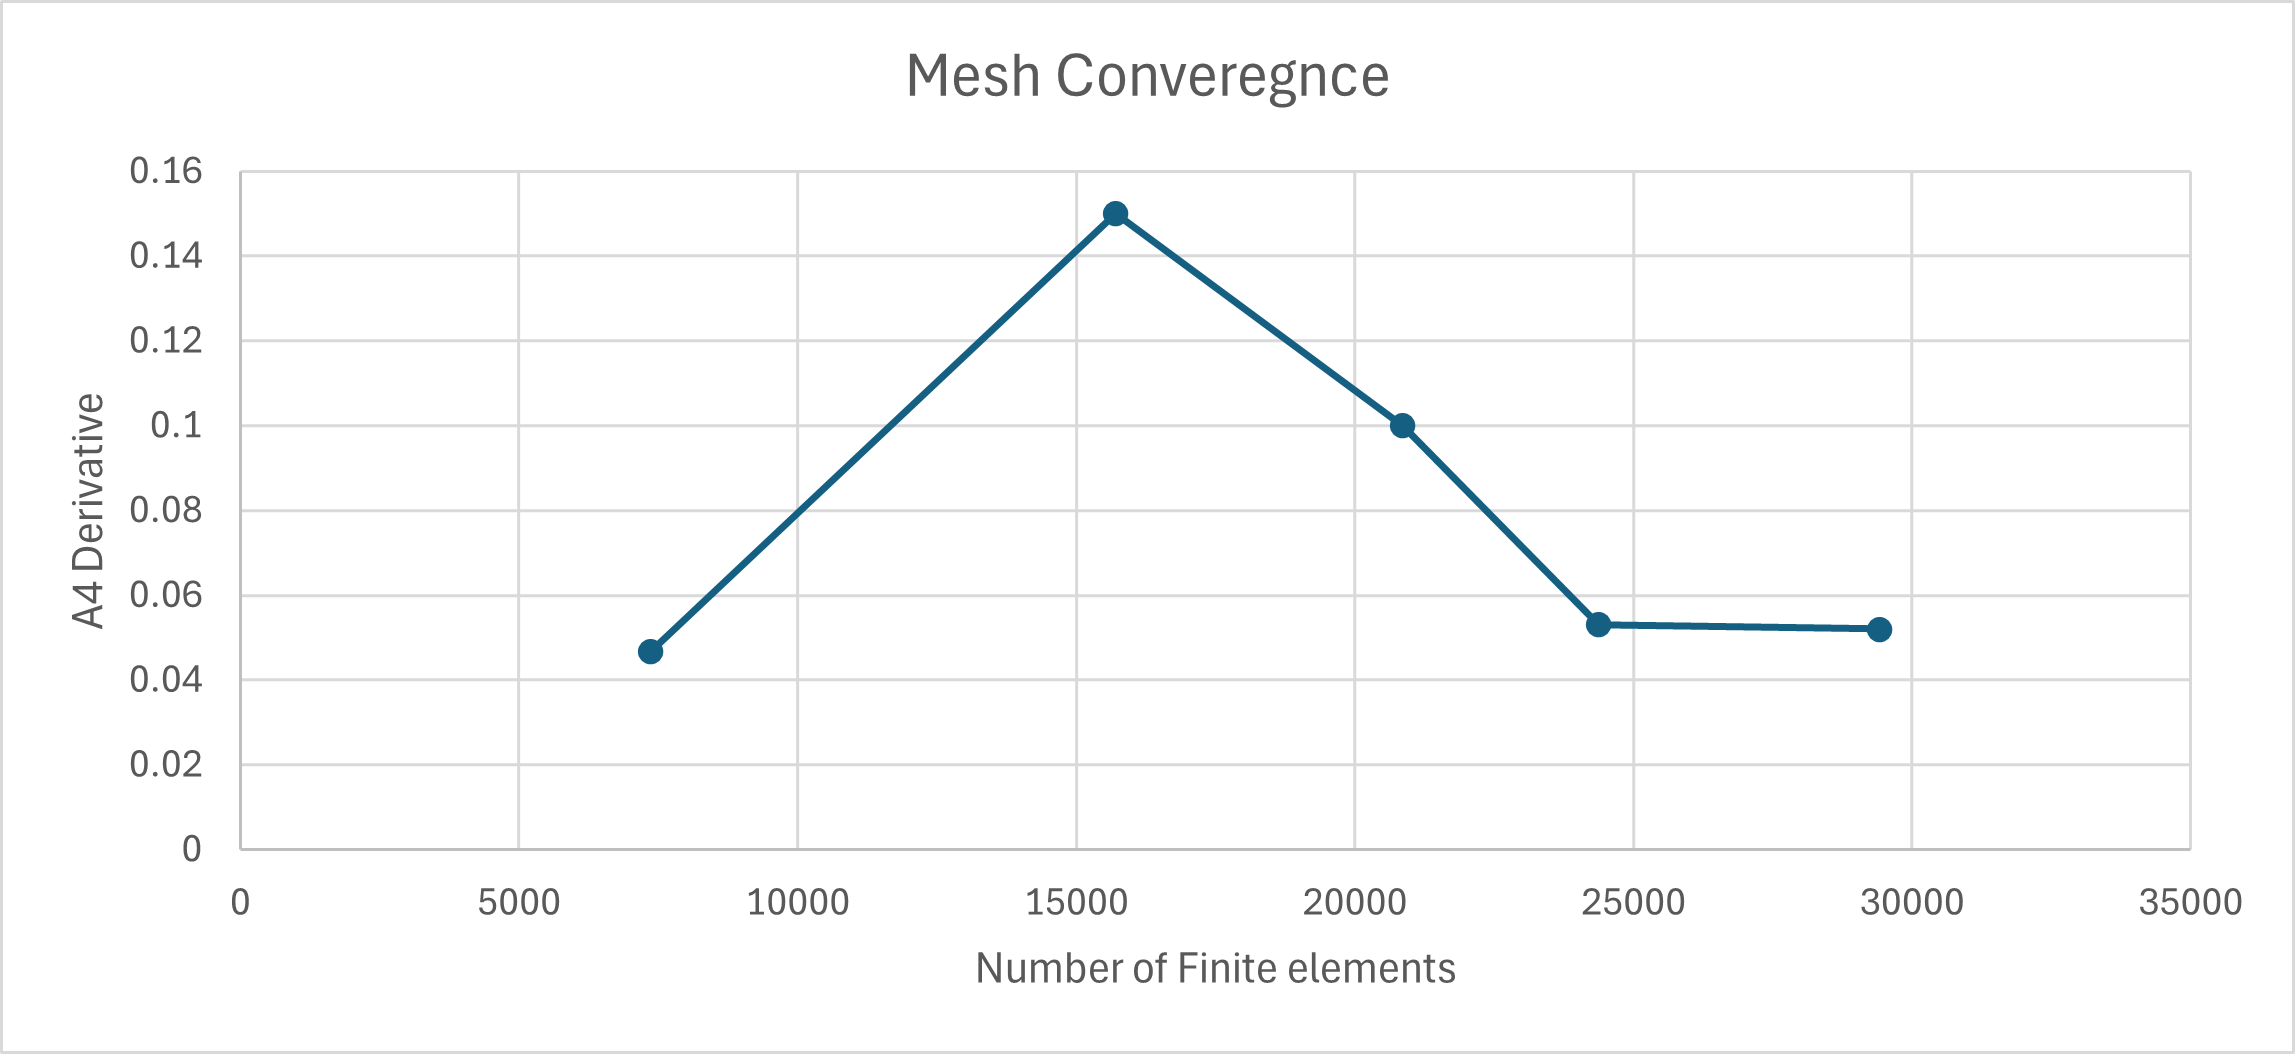
\includegraphics[width=\textwidth]{Figures/Convergence_Study_A4}
        \caption{A4}
        \label{fig:a4}
    \end{subfigure}
    
    \caption{Mesh Convergence Study Results}
    \label{fig:convergence}
\end{figure}

\end{document}
